\documentclass[11pt]{article}
\usepackage{amsmath}
\usepackage{amssymb}
\usepackage{graphicx}
\usepackage[font=small,labelfont=bf]{caption}
\usepackage{subcaption}
\usepackage{float}
\usepackage[font={small}]{caption}
\usepackage{setspace}
\usepackage[margin=30mm]{geometry}
\usepackage{listings}

\usepackage{fancyhdr} % Custom headers and footers
\pagestyle{fancyplain} % Makes all pages in the document conform to the custom headers and footers
\fancyhead{} % No page header - if you want one, create it in the same way as the footers below
\fancyfoot[L]{} % Empty left footer
\fancyfoot[C]{\textit{spline\_slit} Documentation} % Empty center footer
\fancyfoot[R]{\thepage} % Page numbering for right footer
\renewcommand{\headrulewidth}{0pt} % Remove header underlines
\renewcommand{\footrulewidth}{0pt} % Remove footer underlines
\setlength{\headheight}{13.6pt} % Customize the height of the header

%\numberwithin{equation}{section} % Number equations within sections (i.e. 1.1, 1.2, 2.1, 2.2 instead of 1, 2, 3, 4)
%\numberwithin{figure}{section} % Number figures within sections (i.e. 1.1, 1.2, 2.1, 2.2 instead of 1, 2, 3, 4)
%\numberwithin{table}{section} % Number tables within sections (i.e. 1.1, 1.2, 2.1, 2.2 instead of 1, 2, 3, 4)

\newcommand{\horrule}[1]{\rule{\linewidth}{#1}} % Create horizontal rule command with 1 argument of height

\title{	
\normalfont \normalsize 
\textsc{Northumbria University: Mathematics and Information Sciences Solar group} \\ [25pt] % Your university, school and/or department name(s)
\horrule{0.5pt} \\[0.4cm] % Thin top horizontal rule
\huge Spline Slit Code Document \\ % The assignment title
\horrule{2pt} \\[0.5cm] % Thick bottom horizontal rule
}

\author{Krishna Mooroogen\\Oliver Scott\\Dr. Richard Morton} % Your name

\date{\normalsize\today} % Today's date or a custom date

\begin{document}

\maketitle % Print the title
\newpage
\section{Introduction}
The following document provides user documentation for the \textit{spline\_slit.pro} code, developed to create time-distance data from cross cuts perpendicular to the central axis of a feature in order track dynamics. The routine can be applied to both straight and curved features making it a versatile option for solar atmospheric physics where the feature can have a variety of different shapes, e.g., coronal loops, spicules, filaments. The code detailed in this document is developed in IDL for the use in (but not limited to) solar physics research. In this document you will find a step by step guide of the use and execution of the code along with image examples.



The code was initially developed by Oliver Scott as part of a summer project and is maintained and updated by Dr Richard Morton. 

\section{Implementation}

The routine takes as input the coordinates of points along the feature of interest, which are supplied by the user either as an array or by `point and click'. The supplied coordinates are fit with a spline function (\textit{spline\_p}) to achieve a finer resolution of the features coordinates. The level of resolution can be set by the user. Once the spline fit has been obtained, the normal vectors are calculated at approximately equally spaced locations (see notes) along the features - with the distance between vectors able to be modified by the user. The normal vectors are used for the calculation of a cross-cut of certain length, from which time-distance diagrams are obtained. The coordinates of the cross-cut are obtained from a vector equation of the line and the data at the calculated coordinates are extracted via cubic interpolation (\textit{interpolate}). The length of the cross-cut can be specified by the user. 

\section{Capabilities}

The Spline Slit code comes with a number of optional additions that further enhance its use. A summary of the key features of the code are:
\begin{itemize}
   \item Any complex shape of the feature can be fit, if a large enough number of initial coordinates are supplied.
  \item Feature selection can be defined manually with mouse click or by data coordinates.
    \item User defined images can be parsed into the routine for feature selection, e.g. the use of unsharp masking to enhance an image for feature selection but do not wish to use the unsharp masked image for further science.
   \item The user is able to define the spacing between points on the fitted spline curve - see section overview.
  \item Users are able to specify the length of the cross-cut they would like to apply.
  \item Option to use anchor points for complex shapes - only designed for implementation with fitting features that are semi-elliptical.
   \item Over plotting of normal vectors to show direction of time distance diagram/cross cut.
\end{itemize}

\section{Overview}
\subsection{Basic Use}

The following code segment describes the most basic use of Spline Slit. 

\lstinputlisting[language=IDL,lastline=2]{laidl.pro}

\noindent Here, ``data" is the input and must be a data cube (x,y,t). It is important for the user to note that large data cubes will take longer to process and therefore is advised for a suitable region of interest (ROI) to be first defined before input. The displayed image is a summed image over the data time frames. The summed image gives the user an approximate ``feel" for where the feature appears most in time. The Keyword \texttt{slits} and the receiving variable ``td" will output the resulting time-distance diagrams. Entering the above code into the IDL terminal will result in a terminal prompt reading, ``Please select 6 points to make track" and an image plot to the screen with the summed input ROI displayed. The number of points used for fitting is specified via the \texttt{pickn} keyword.

%#####################################################################
\begin{figure}[t!]
\centering
\begin{subfigure}{7cm}
\includegraphics[scale=0.47, clip=true, viewport=1.5cm 1cm 18cm 13cm]{firstplot}
\caption{ROI image before point selection, the image is summed over the time frames available in the data cube.\tiny}
\label{firstplot}
\end{subfigure}
\hfill    
\begin{subfigure}{7cm}
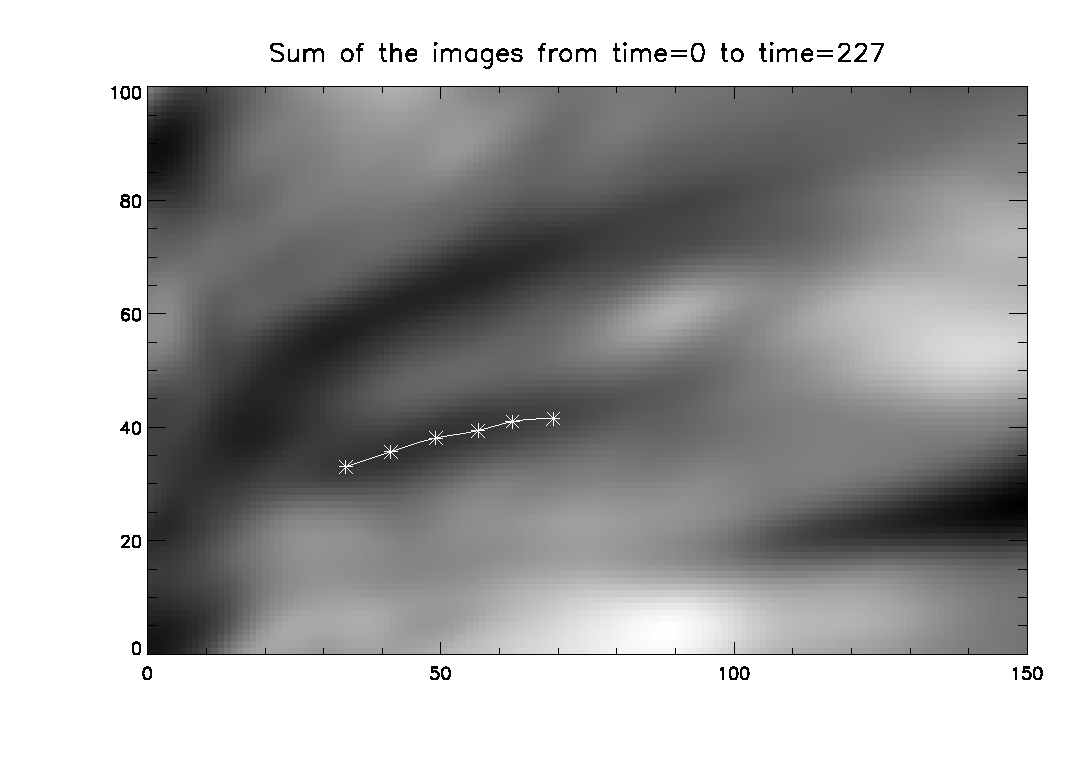
\includegraphics[scale=0.47, clip=true, viewport=1.5cm 1cm 18cm 13cm]{secondplot}
\caption{ROI summed image after the 6 points have been selected, the white line shows the polynomial fit through the 6 points across the axis of the selected feature.\tiny}
\label{secondplot}
\end{subfigure}
\caption{ROI images of before and after point selection. Dark fibrils can be seen in the image which are the target of interest.\tiny}
\end{figure}
%#####################################################################

After selecting six points with the mouse, the points will be fit with a spline. This will serve as the guideline along the features axis, to which perpendicular  cross-cuts will be calculated. The user is advised to use six points minimum for the guideline where available. The number of points is defined with the keyword \texttt{pickn}. The terminal prompt will change the requested number of points reflecting the input in the keyword \texttt{pickn}.

The output ``td" will be a data cube of intensity time-distance diagrams for the number of cross-cuts number along spline track. The number of time- distance diagrams depends on the number of points input or the spacing set by the \texttt{spacing} keyword. The routine will make a cross-cut at every available position in the fitted spline if the \texttt{spacing} keyword is not set. If the \texttt{spacing} keyword is set, it imposes a separation distance between each cross cut. It is suggested the user experiment with this feature to grasp the idea.

\medskip
It is important to note that due to the way the \textit{spline\_p} routine works in IDL the spacing between points will not exactly match the spacing interval set in the keyword. An estimate of the spacing can be obtained by calling the \texttt{curvepoints} keyword to obtain the x,y coordinates of the spline. To achieve an actual spacing as close as possible to the desired spacing, it is preferential to use the \texttt{oversample} keyword. This oversamples the spline fit increasing the point density and, using a linear approximation for the distance between spline points, cumulatively sums the inter-spline-point distance till the total length reaches the desired spacing. The more the curve is oversampled, the greater the accuracy of the linear approximation and also the desired spacing. Oversampling by a factor of two or three usually gives a reasonable accuracy, i.e. to 2-3 decimal places. The time for the routine to run obviously increases as the amount of oversampling increases. The keyword should be called as, e.g., \texttt{oversampling=2} for an increase of $10^2$ number of spline points.

%#####################################################################
\begin{figure}[t!]
\centering
\begin{subfigure}{7cm}
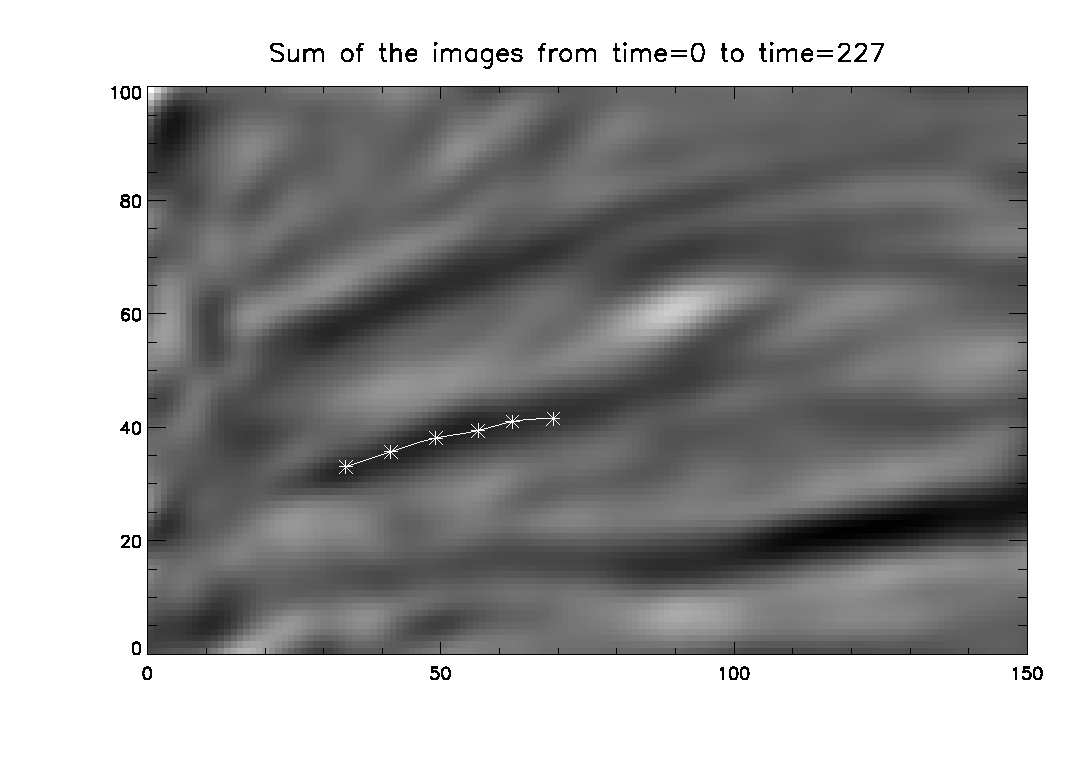
\includegraphics[scale=0.47, clip=true, viewport=1.5cm 1cm 18cm 13cm]{unsh}
\caption{ROI unsharped masked image supplied by user by the \texttt{intim} keyword. \tiny}
\label{unsh}
\end{subfigure}
\hfill    
\begin{subfigure}{7cm}
\includegraphics[scale=0.47, clip=true, viewport=1.5cm 1cm 18cm 13cm]{vec}
\caption{ROI summed image between the time frames 0 and 227. Over plotted is the normal vectors showing the direction of the time distance diagrams along the feature.\tiny}
\label{vec}
\end{subfigure}
\caption{ROI images showing the use of the  optional keywords.\tiny}
\end{figure}
%#####################################################################

\newpage
\subsection{Example}
The following examples details a more advanced use of the routine using the optional keywords. 

\lstinputlisting[language=IDL,firstline=5,lastline=7]{laidl.pro}

Here the keyword \texttt{intim} has been used to specify an unsharp masked image to use as a guide when selecting the spline points. The \texttt{distance} keyword is used to specify the length of the cross cut. The \texttt{gpoints} and \texttt{curvepoints} keywords output the data points of the selection points and the data points of the spline curve respectively. The \texttt{frames} keyword has been used here to define the time interval in which the display image will be summed over.

\lstinputlisting[language=IDL,firstline=3,lastline=5]{laidl.pro}

Here the \texttt{vector} keyword displays the normal vector on the plot indicating the direction of the time distance diagram.



%#####################################################################
\begin{figure}[t!]
\centering
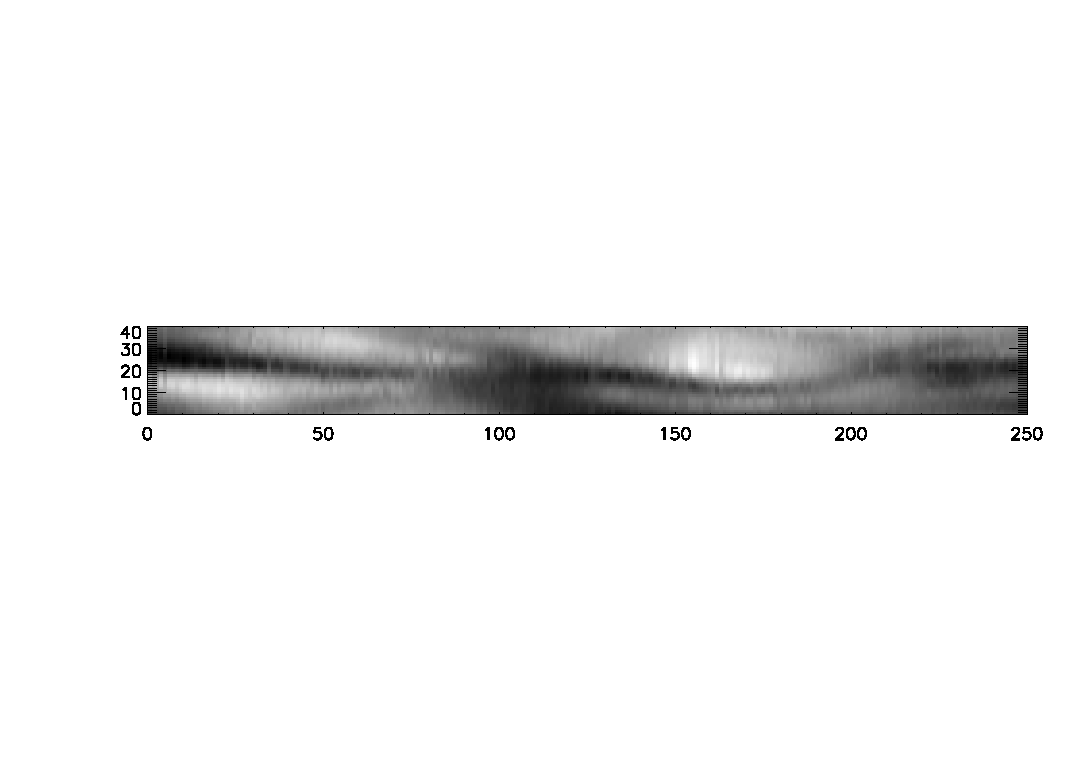
\includegraphics[scale=1, clip=true, viewport=1.5cm 5cm 18cm 8cm]{td}
\caption{Image showing time distance diagram as an output of the routine. The image has been rotated and the aspect ratio increased.\tiny}
\label{td}
\end{figure}
%#####################################################################

\newpage
\subsection{Optional Keywords}

Here we list the optional keywords and their purpose.  
\begin{itemize}
\item Inputs

\textit{distance} - Integer value variable. Sets the half length of the time distance slit, the default is set as ten. Change this variable to change displacement length of the time distance diagram. 

\textit{frames} - The image used for point selection is an average of entire data set, enter array [t1,t2] to select specific frames for averaging. Input should be integer array within limits of data's third dimension.

\textit{pickn} - If set, will use the procedure \texttt{pick\_n} to enable the user to select points by clicking on an image. This should be set to an integer value of the number of points required to spline to. For example setting the value \texttt{pickn=6}, the routine will expect the user to click to define six points on the feature of interest.
                   
\textit{gpoints} - Specifies guide values for/from the spline fit. Can be used as an input or an output. As an input, give the spline points values instead of picking them with \texttt{pickn}. The value of \texttt{gpoints} must be an integer array of dimensions (N,2). If both \texttt{gpoints} and \texttt{pickn} are set, the values of \texttt{gpoints} will be ignored and overwritten. As an output, returns the values from the picking of points used with the \texttt{pickn} routine.

\textit{vector} - Over plots normal vectors to the existing plot indicating the direction of the time distance diagram along the curved guideline.

\textit{spacing} - Integer scalar value that gives the spacing between points on the fitted curve. If unset, the default spacing will be used in accordance with the IDL routine \texttt{spline\_p}. NOTE: \texttt{spline\_p} intervals typically do not give the desired spacing value (normally smaller values). To get intervals close to desired spacing, use the oversample keyword. 

\textit{oversample} - Over samples the curve in \texttt{spline\_p} by $10^oversample$ - obviously large values of oversample will take a long time.

\textit{anchor} - Will use first and last selected points as anchor points for defining a curve, not used in slit extraction. 

\textit{intim} - User supplied image to use for picking the guide points. For example if the user would like to use a filtered image to track the feature but does not want to use the filtered image in the time distance diagram.

\item Outputs

\textit{curvepoints} - Outputs the spline data points.

\textit{slits} - Cube of time distance diagrams (displacement, time and time distance number).

\textit{gpoints} - As an output when used in combination with the \texttt{pickn} keyword, the output variable will contain the data points of the selected guide points.

\end{itemize}



\section{Notes}

Care needs to be taking with selecting points for the tracking. Clicking on the edge of the display window will register with the routine as a location. So, when switching computer windows ensure you click the grey bar above the x11 window and not on the plot area. 



The default output will be displacement, time and time distance number and therefore the user may wish to rotate the time distance diagram. Depending on the slit length the aspect of the resulting plot may need changing to be visible.



Designed for time distance but in reality will work with any cube therefore can be utilised interestingly for different cases of tracking an image over the third image dimension.


\end{document}